\section{Implementierung}
\label{sec:implementation-analysis}

Dieses Kapitel beschreibt den Implementierungsprozess von esqulino und erläutert einige technische Entscheidungen. Sofern sich während der Entwicklung Ideen für bisher nicht bedachte Funktionalität ergaben, wurden diese in Anlehnung an den "`Minus 100 Points"'-Artikel von Eric Gunnerson \cite{gunnerson-minus-100} geprüft.

\todo[inline]{Mehrere Datenbanken je Projekt, CSV-Import}

\subsection{Client-Server-Architektur}

Der softwaretechnische Unterbau der Entwicklungsumgebung setzt auf aktuelle Webtechnologien auf (siehe \ref{sec:req-web-application}~\nameref{sec:req-web-application} für die Diskussion der Begründung) und teilt sich in zwei distinkte Codebasen für Server und Client.

\begin{description}
\item[Server: Ruby mit Sinatra] \hfill\\
  Die Aufgaben des Servers sollen sich konzeptionell möglichst auf die Auslieferung und Speicherung von Daten beschränken. Die Interaktion findet dabei primär über eine REST-artige JSON Schnittstelle statt, serverseitig gerendert werden lediglich die Projekte der Schüler.
\item[Client: Typescript mit Angular 2] \hfill\\
  Aufgrund des hohen Grades an Interaktivität bietet sich eine rein clientseitige Visualisierung an, die weitestgehend auf Roundtrips zum Server verzichtet. Außer für den Zugriff auf serverseitige Resourcen (Datenbank, gespeicherte Ressourcen, gerenderte Seiten) werden alle Operationen im Browser ausgeführt.
\end{description}

\begin{figure}[p]
  \centering 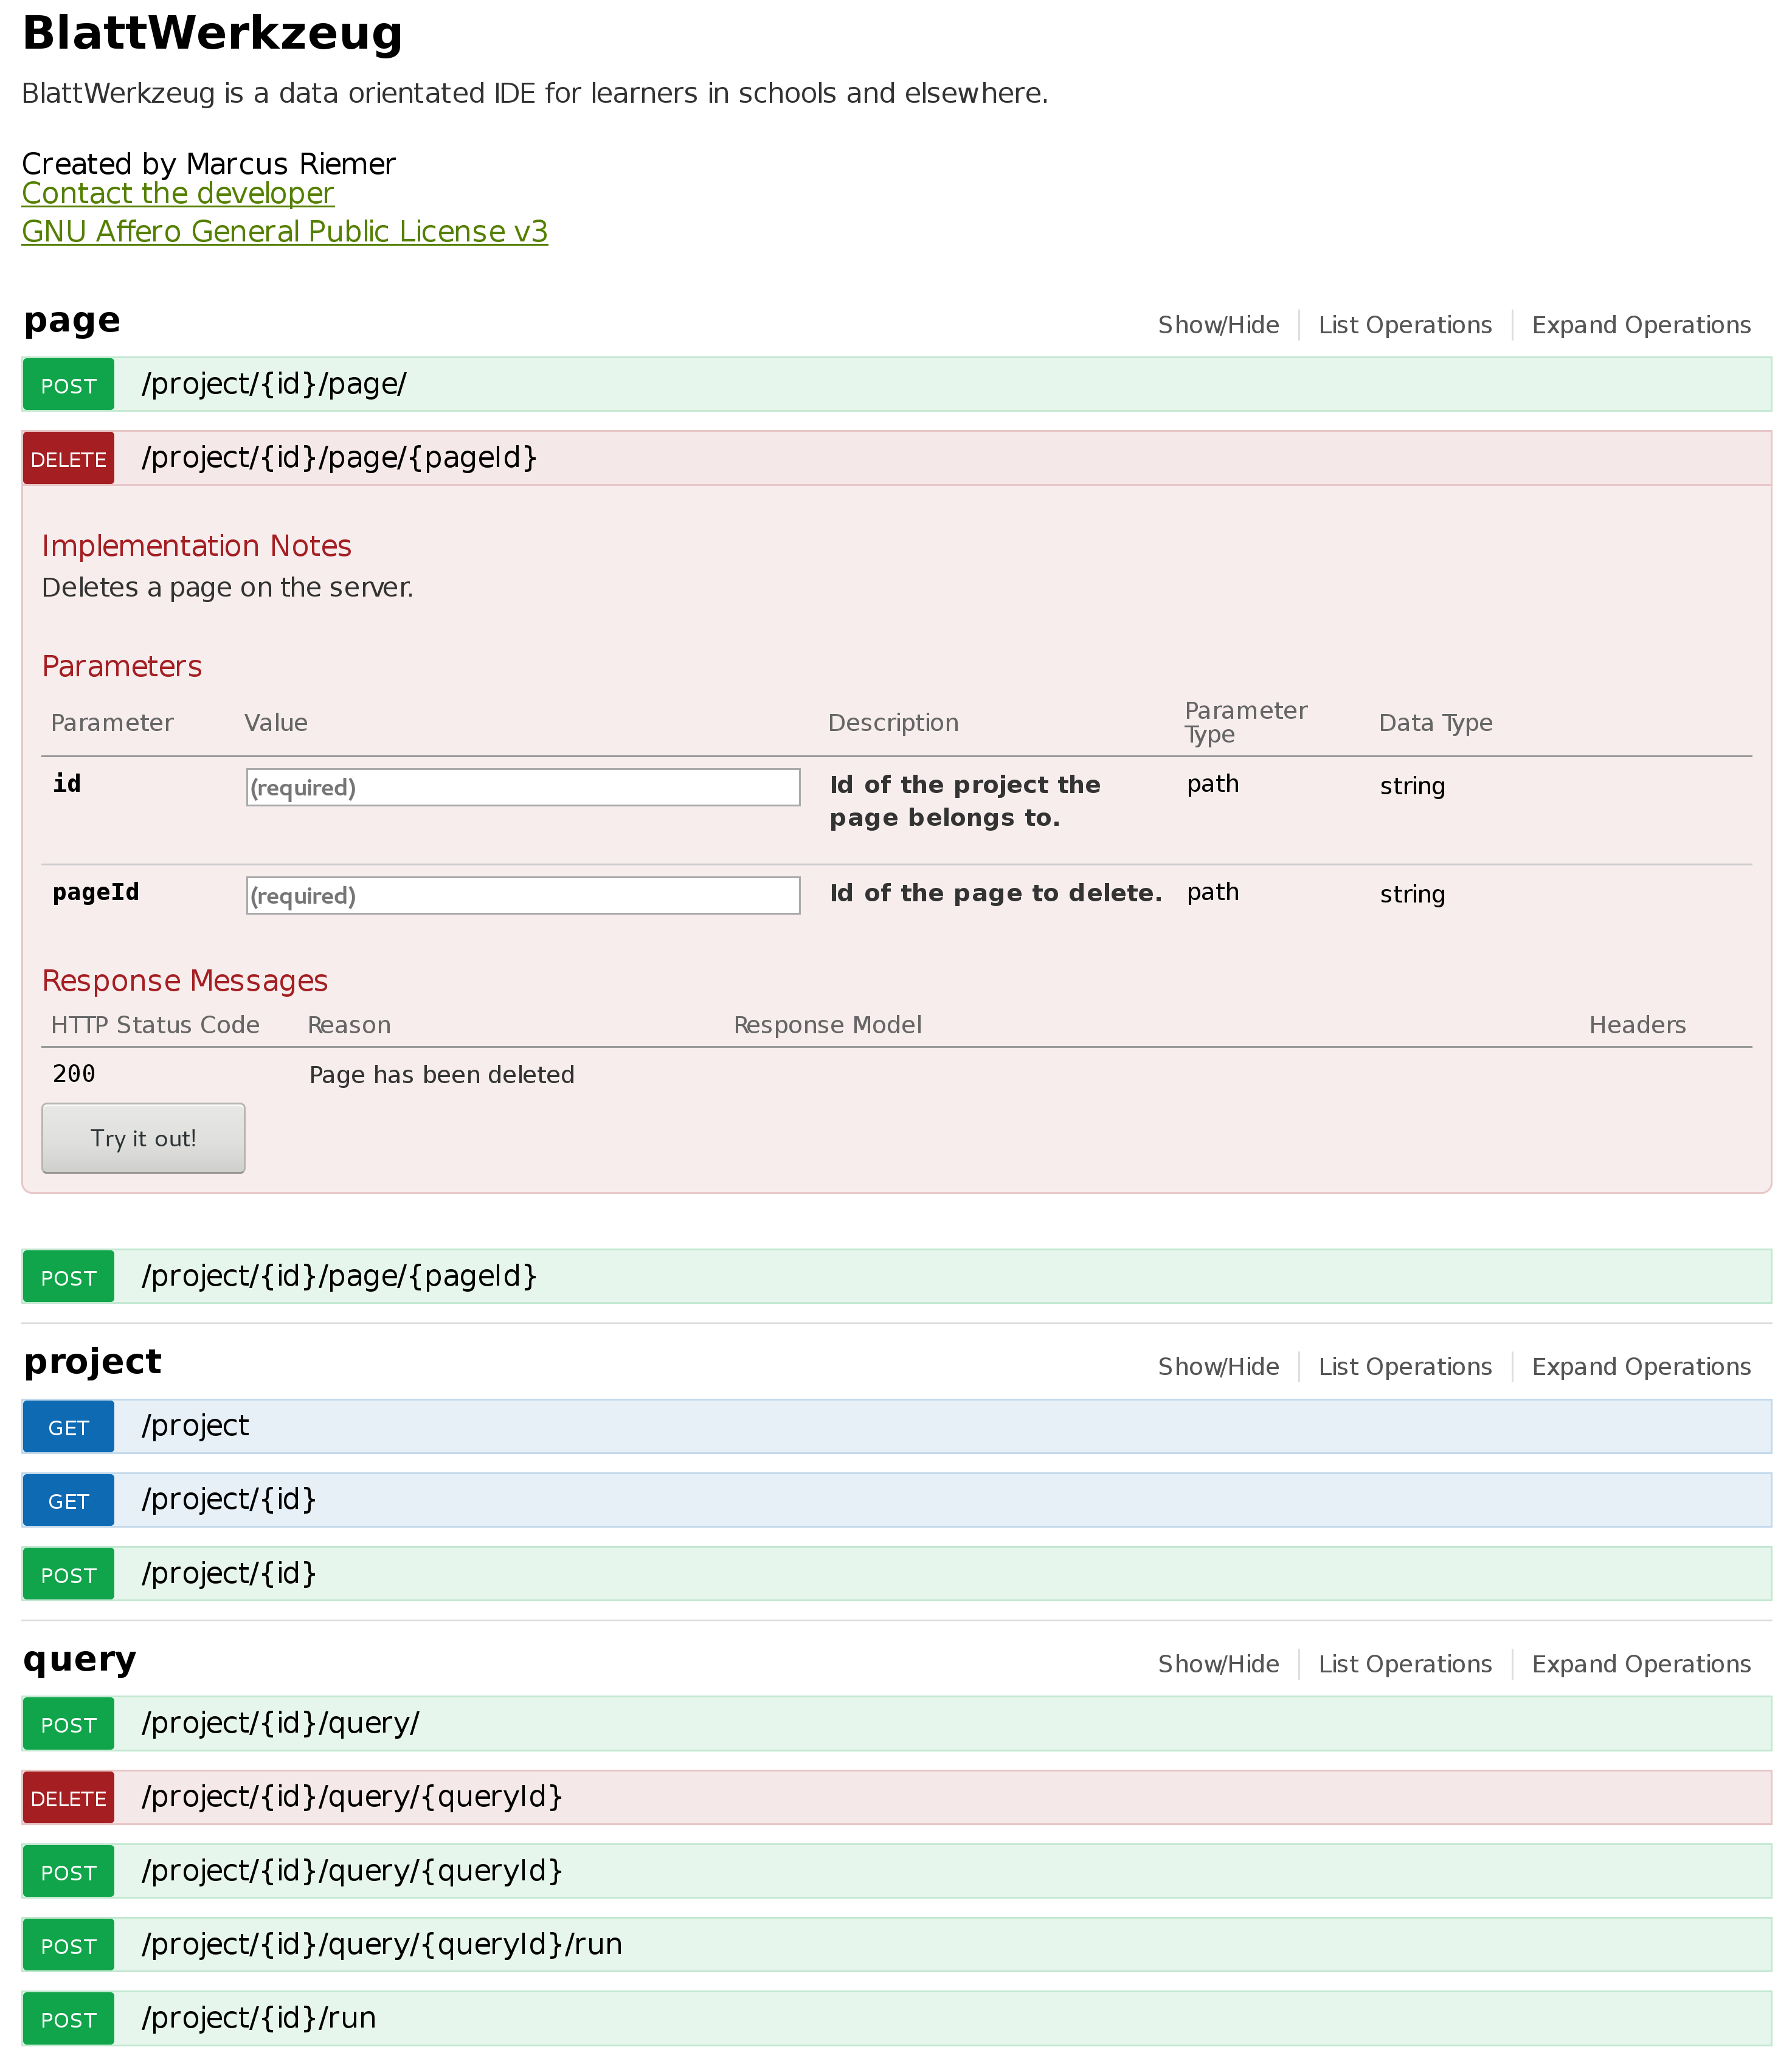
\includegraphics[width=\textwidth]{images/openapi-query-example.png}
  \caption{Generiert aus der Spezfikation: API-Browser für esqulino}
  \label{fig:openapi-query-example}
\end{figure}

Um die Schnittstelle zwischen diesen beiden Komponenten so transparent wie möglich zu halten, werden diese gemäß der OpenAPI Spezifikation \cite{open-api} dokumentiert. Dieses offene Format ermöglicht es auf eine hilfreiche Auswahl an standarisierten Tools aufzubauen. Zum Beispiel können aus der Spezifikation interaktive Testumgebungen für die Server-Schnittstellen erzeugt werden, Abbildung \ref{fig:openapi-query-example} zeigt ein Beispiel dafür.

Als primäres Interface für die Kompilierung wird ein \lstinline{Makefile} genutzt. Dieses prüft ob auf dem aktuellen System alle nötigen Abhängigkeiten verfügbar sind und stellt sicher, dass Übersetzungsschritte nur ausgeführt werden, wenn sie tatsächlich notwendig sind. Von den technischen Details der unterschiedlichen Programmierumgebungen aufgrund der unterschiedlichen Programmiersprachen kann so außerdem elegant abstrahiert werden: Ein Programmierer kann sich die exakten Aufrufe der unterschiedlichen Paketmanager zwar anschauen, wird im Normallfall aber nur \lstinline{make install-deps} aufrufen.

\subsection{Meilensteine}

Der Editor für Datenbankabfragen versprach im Vergleich zum Seiteneditor das einfachere Teilprojekt zu sein: Die Struktur einer Abfrage ist sehr strikt festgelegt, der Umfang lässt sich gut lokal eingrenzen. Im ersten Schritt wird allerdings nicht der komplette Editor implementiert, sondern zunächst nur das interne Datenmodell für die Abfragen in Form eines abstrakten Syntaxbaumes mitsamt den dazugehörigen Tests.

Um den Umfang des Prototypen zu Begrenzen, wurde die Implementierungsphase anhand der folgenden funktionalen Meilensteine geplant:

\begin{description}
\item[Bearbeitung von Projektdaten] \hfill \\
  Schwerpunkt dieses Meileinsteins ist Implementierung grundlegender gemeinsamer Schnittstellen. Diese müssen auf vom Server als HTTP-Endpunkte angeboten und vom Client angesprochen werden können.
  \begin{itemize}
  \item Persistierung von Projekten mit Name und Beschreibung
  \item Editor für Projekteigenschaften
  \item Auflistung aller Projekte einer esqulino-Instanz
  \end{itemize}
\item [Anzeige eines Datenbankschemas] \hfill \\
  Neben der funktionalen Anforderung umfasst dieser Meilenstein die Erweiterung des Clients um die typischen Bestandteile des Benutzerschnittstelle einer Entwicklungsumgebung. Serverseitig erfordert dieser Meilenstein zum ersten Mal eine Verbindung mit der Datenbank.
  \begin{itemize}
  \item Editor zur Anzeige eines Datenbankschemas
  \item Seitenliste mit Übersicht über alle Bestandteile eines Projekts
  \item Toolbar mit Knöpfen, deren Verfügbarkeit vom aktuellen Editor abhängt
  \item Wechsel zwischen verschiedenen Editoren
  \end{itemize}
\item [Datenmodell für Abfragen] \hfill \\
  Der abstrake Syntaxbaum für Datenbankabfragen in esqulino sowie die dazu passenden Testfälle.
  \begin{itemize}
  \item Einfache Projektion durch Auswahl von Spalten im \texttt{SELECT}
  \item Kreuzprodukte unterschiedlicher Tabellen im \texttt{FROM}
  \item Einschränkungen der Ergebnismenge mit Ausdrücken im \texttt{WHERE}
  \item Ausdrücke mit binären Operationen zwischen Spalten, Konstanten und benutzerdefinierten Werten.
  \end{itemize}
\item [Editor für Abfragen] \hfill \\
  Implementierung des Drag \& Drop Editors für SQL-Abfragen und Vorschau der Ergebnisse.
  \begin{itemize}
  \item Drag \& Drop Editor für Abfragen
  \item Ausführung von SQL-Abfragen auf dem Server
  \item Clientseitige Anzeige von serverseitigen Ergebnissen
  \end{itemize}
\item [Datenmodell für Webseiten] \hfill \\

\item [Editor für Webseiten] \hfill \\

\item [Qualitätssicherung] \hfill \\
  
\end{description}

\subsection{Datenbanksystem}
\label{sec:implementation-database-system}

Die Wahl des konkreten Datenbanksystems hat einen unmittelbaren Einfluss auf nahezu alle Bereiche von esqulino. Im einzelnen handelt es sich dabei um die exakte Variante der SQL Syntax, auf die Rahmenbedingungen für den Betrieb der Entwicklungsumgebung und auch auf die Fortführung der Projekte mit externen Programmen.

Die in der Praxis häufig dominierenden Entscheidungskriterien der Skalierbarkeit, die Unterstützung unterschiedlichster Zugriffsrechte und auch die allgemeine Performance spielen nur eine sehr untergeordnete Rolle. Die zu erwartenden Datenbeständen sollten normalerweise im Bereich nur einiger Megabyte liegen und die in der Praxis möglicherweise einzige Unterscheidung von Zugriffsrechten wäre zwischen lesendem und schreibenden Zugriff. Für die Wahl des Datenbanksystems werden stattdessen die folgenden Kriterien gewählt und hinsichtlich ihrer Relevanz sortiert:

\begin{description}  
\item[Kostenlose Verfügbarkeit] \hfill \\
  Der Betrieb des Datenbanksystems soll nicht mit Lizenzkosten für Schulen, Lehrkräft, Lernende oder auch freiwillige Entwickler verbunden sein.
\item[Einfacher Betrieb] \hfill \\
  Zwar ist für den Einsatz von esqulino aufgrund des Browsers als Client schon die Nutzung eines Servers nötig, das Datenbanksystem sollte den Betrieb dennoch nicht mehr als unbedingt notwendig weiter verkomplizieren. Eine wesentliche Rolle spielt dabei die Platformunabhängigkeit: Das Datenbanksystem sollte, wie auch der esqulino Server, auf jedem gängigen Betriebssystem lauffähig sein.
\item[Einfache Backups] \hfill \\
  Die gewünschte Exportfunktion für Projekte macht es nötig, den gesamten Datenbestand vergleichsweise einfach exportieren und importieren zu können. Darüber hinaus sollte es auch für Lehrkräfte möglichst einfach sein mit allen Projekten zu einem anderen esqulino-Server umzuziehen.
\item[Tools zur Modellierung] \hfill \\
  Da diese Arbeit sich nicht mit der Datenmodellierung befasst, muss das entsprechende Datenbankschema extern erzeugt werden. Von einer guten Unterstützung für Modellierungsvorhaben profitiert dementsprechend indirekt auch esqulino.
\item[Tools zur Entwicklung von SQL-Abfragen] \hfill \\
  Sobald ein Entwickler an die Grenzen des SQL-Editor von esqulino stößt, soll es so einfach wie möglich sein die Abfragen in einem externen Editor zu schreiben und danach in Textform wieder an esqulino zu übergeben.
\end{description}

Das Kriterium der ``kostenlosen Verfügbarkeit'' ist dankenswerterweise sehr einfach zu erfüllen: Es existiert eine Vielzahl von praktisch eingesetzten quelloffenen Datenbanksystemen. Die Kriterien ``einfacher Betrieb'' und ``einfache Backups'' teilen die denkbaren Systeme recht eindeutig in zwei Lager: Eingebette Datenbanken lassen sich sehr einfach betreiben und sichern. Das starten eines weiteren SQL-Server-Prozesses ist bei dieser Betriebsart nicht nötig, der Im- oder Export des gesamten Datenbestandes erfordert nur das kopieren einer einzigen Datei.

Um den Betrieb folglich so einfach wie möglich zu halten, wurden für esqulino zunächst eingebettete Datenbanksysteme betrachtet. Aus der Masse an verfügbaren Systemen sticht das SQLite-System jedoch sehr weit hinaus: Der Quelltext ist gemeinfrei, der Betrieb sogar auf exotischen Systemen möglich und es existiert eine Fülle von verschiedensten Programmen für alle Betriebssysteme.

\unsure[inline]{Theoretisch ist die Menge an denkbaren Systemen fast unüberschaubar groß, praktisch sticht SQLite aus der Masse an Optionen heraus. Wie ausführlich muss ich das begründen?}

\subsection{Tests}

Die Funktionalität der, relativ isolierten und daher gut zu testenden, internen Datenmodelle samt den darauf definierten Operationen wird über Unit-Tests sichergestellt. Diese Tests können einfach in jedem Browser ausgeführt werden und eignen sich daher auch um im Zweifelsfall unterschiedliche Verhaltensweisen verschiedener Browser zu erfassen.

Als technisches Fundament wird für diese Testfälle auf der Jasmine-Bibliothek aufgebaut. Zu prüfende Zusicherungen werden durch Verkettung zweier Funktionen ausgedrückt: \lstinline{expect().toEqual()}. Neben \lstinline{toEqual()} sind natürlich auch andere Vergleiche wie \lstinline{isUndefined()} möglich. Wenn innerhalb eines Testfalls auch nur eine einzige dieser Prüfungen nicht zu \lstinline{true} auswertet, wird der Testfall als ingesamt fehlgeschlagen markiert. Im Falle von mehreren gescheiterten Prüfungen sind werden dabei alle unerwarteten Ergebnisse aufgelistet.

listing \ref{lst:unit-test-example} illustriert, wie die meisten testfälle in esqulino aufgebaut sein. jeder testfall beginnt mit der definition eines datenmodells und endet mit testfällen für die korrekte serialisierung. ganz konkret existiert also in jedem testfall eine variable \lstinline{model}, welche im konstruktor der zu testenden klasse zum einsatz kommt und in nicht-mutierenden testfällen als ergebnis der \lstinline{tomodel()} methode reproduziert werden muss. formal ausgedrückt handelt es sich es sich bei der verkettung des konstruktors mit der \lstinline{tomodel()}-methode also um eine neutrale operation.

die dateien mit den unit-tests liegen im dateisystem immer "`neben"' ihren implementierungen, der dateiname wird allerdings mit dem suffix \lstinline{spec} wie "`specification"' ergänzt. das beispiel in listing  \ref{lst:unit-test-example} wurde der datei \lstinline{select.spec.ts} entnommen, der code für die zu testende funktionalität findet sich folglich in \lstinline{select.ts}.

\lstinputlisting[
  language=javascript,
  caption=unit-test für eine korrekte \lstinline{select}-abfrage,
  label=lst:unit-test-example,
  float,floatplacement=p,
  numbers=left
]{snippets/unit-test-example.ts}

die serverseitige funktionalität wird aktuell ausschließlich über "`ende-zu-ende"'-tests mit einem speziell instrumentierten browser geprüft. für diese tests ist ein speziell vorbereitetes testprojekt in einem exakt definierten zustand sowie neben dem browser auch ein esqulino-server notwendig.

\subsection{struktur eines projekts}

die grundsätzliche struktur eines esqulino-projektes wird in diagramm \ref{uml:class-diagram-core-entities} ersichtlich. diese darstellung visualisert nicht die konkrete implementierung des servers oder des clients, sondern illustriert die grundlegenden beteiligten datenstrukturen. jede dieser entitäten, also sowohl projekte als auch ihre ressourcen, enthält eine eigene versionsangabe. dadurch kann auf jede veränderung an dieser struktur explizit eingegangen werden (\ref{sec:implementation-migration}~\nameref{sec:implementation-migration}), aktuell laden sowohl server als auch client nur ressourcen deren version exakt passt.

jede ressource (\lstinline{projectresource}) verfügt über eine interne id sowie einen sprechenden namen. in der aktuellen version von esqulino handelt es sich bei dieser id um eine \lstinline{guid}, sollte also weltweit einzigartig sein. theoretisch wäre es dadurch denkbar diese ressourcen auch zwischen projekten zu kopieren bzw. zu teilen. intern werden referenzen auf ressourcen immer anhand der id referenziert. eine umbenennung von ressourcen durch den benutzer hat daher keine auswirkungen auf etwaige referenzen an anderer stelle.

\begin{diagram}[p]
  \begin{tikzpicture}
    \begin{interface}[text width=7cm]{apiversionable}{-4, 0}
      \attribute{apiversion : string}
    \end{interface}
    
    \begin{class}[text width=7cm]{project}{-8, -4}
      \implement{apiversionable}
      
      \attribute{id : string}
      \attribute{name : string}
      \attribute{description : string}
      \attribute{indexpageid : string}
    \end{class}

    \begin{abstractclass}[text width=7cm]{projectresource}{0, -6}
      \implement{apiversionable}
      
      \attribute{id : string}
      \attribute{name : string}
    \end{abstractclass}

    \begin{class}[text width=7cm]{page}{0, -10}      
      \attribute{body: bodynode}
      \attribute{referencedqueries: queryreference[]}
      \attribute{parameters: pageparameter[]}
    \end{class}

    \begin{class}[text width=7cm]{query}{0, -14}
      \attribute{select : select}
      \attribute{delete : insert}
      \attribute{insert : insert}
      \attribute{update : update}
      \attribute{from   : from}
      \attribute{where  : where}
    \end{class}

    % query and page implement projectresource
    \draw[->] (query.east) -- ++ (1,0) -- ($(projectresource.east)+(1,0)$) -- (projectresource.east);
    \draw[-] (page.east) -- ++ (1,0);

    % each resource has a reference to the project
    \draw[] (projectresource.north)  |- (project.east);
    \node[xshift=0.3cm, yshift=0.3cm] at (projectresource.north) {n};
    \node[xshift=0.3cm, yshift=0.3cm] at (project.east) {1};
    
    % a project has pages ...
    \draw[] (page.west)  -| (project.south);
    \node[xshift=0.3cm, yshift=-0.5cm] at (project.south) {1};
    \node[xshift=-0.5cm, yshift=0.3cm] at (query.west) {0..n};
    \node[xshift=-2.5cm, yshift=0.3cm] at (query.west) {queries};

    % ... and queries.
    \draw[] (query.west) -| (project.south);
    \node[xshift=-0.5cm, yshift=0.3cm] at (page.west) {0..n};
    \node[xshift=-2.5cm, yshift=0.3cm] at (page.west) {pages};
  \end{tikzpicture}

  \caption{abstrakte übersicht über die ressourcen eines projektes}
  \label{uml:class-diagram-core-entities}
\end{diagram}

\subsection{serverseitige persistenz}
\label{sec:implementation-persistence}

grundsätzlich sollte die serverseitig persistierte version einer resource möglichst identisch mit dem übertragungsformat sein, konkret persistiert werden also json-dokumente. bei der auslieferung müssen dann lediglich sensible informationen gefiltert werden, in der datenstruktur der jeweiligen implementierung sollte diese felder daher als optional betrachtet werden. sofern jedoch keine filterung notwendig ist, können diese dokumente einfach unverändert bereitgestellt werden.

um json-dokumente serverseitig zu persistieren kommen im wesentlichen zwei speichermethoden in frage: entweder werden datensätze direkt als datei im dateisystem abgelegt oder in einer dokumentenorientierten datenbank gespeichert.

bei einer speicherung im dateisystem wäre der rein lesende zugriff auf esqulino-datensätze sogar mit einem einfachen webserver für statische dateien möglich. um ein projekt anzusehen oder zu editieren reicht ein normaler texteditor, neue projekte können einfach per copy \& paste im dateisystem angelegt werden. perspektivisch wäre es relativ einfach möglich ein projekt mit gängigen versionsverwaltungsprogrammen wie git oder mercurial zu versionieren.

die speicherung in dokumentenorientierten datenbank wie mongodb oder in einem key/value-store wie redis macht den zugriff auf die persistierten daten abhängig von einem externen serverprozess. der universelle zugriff über das dateisystem weicht einem speziellem programm zur navigation innerhalb der jeweiligen datenbank. mit dieser komplexität gewinnt man eine wesentlich größere flexibilät in bezug auf horizontale skalierung.

technisch gesehen ist ein projekt also eine sammlung von dateien in einer festgelegten ordnerstruktur.

\begin{diagram}
  \dirtree{%
    .1 empty-project/.
    .2 queries/.
    .2 pages/.
    .2 config.yaml.
    .2 db.sqlite.
  }
  \caption{leeres projekt}
\end{diagram}

bei der \texttt{config.yaml} handelt es sich aus im nachhinein unsinnigen gründen um eine yaml-datei.

\subsection{Hinweise zum Client}

Der verwendete Typescript Compiler hat zum Zeitpunkt der Anfertigung dieser Arbeit einen bekannten Bug in der Codegenerierung \cite{ts-compiler-class-order-bug} um den wiederholt herumgearbeitet werden musste. Konkret äussert sich dieser Fehler, wenn die Definition der Oberklasse einer sich davon ableitenden Klasse erst im Nachhinein erfolgt (Listing \ref{lst:ts:class-order-bug}). In diesem Fall kommt es zu keiner Warnung durch den Compiler, sondern zu einem Laufzeitfehler im kompilierten Javascript-Code.

\lstinputlisting[language=JavaScript,caption=Falsche Reihenfolge der Klassendefinition, label=lst:ts:class-order-bug]{snippets/class-inheritance-order-bug.ts}

\subsection{Administration}
\label{sec:implementation-administration}

Momentan aufgrund von Zeitmangel nur in Form der Kommandozeilenschnittstelle.

\subsubsection{Schema-Migrationen}
\label{sec:implementation-migration}

%%% Local Variables:
%%% mode: latex
%%% TeX-master: "thesis"
%%% End:
